\documentclass[12pt]{book}
\usepackage[utf8]{inputenc}
\usepackage{graphicx}
\usepackage[a4paper,width=150mm,top=25mm,bottom=25mm,bindingoffset=6mm]{geometry}
\usepackage[utf8]{inputenc}
\usepackage[T1]{fontenc}
\usepackage[english]{babel}
\usepackage{setspace}
\usepackage{amsmath}
\usepackage{amssymb}
\usepackage{amsfonts}
\usepackage{bm}
\usepackage{fancyhdr}
\usepackage[round]{natbib}
\usepackage{algorithmicx}
\usepackage{algorithm}
\usepackage[noend]{algpseudocode}
\usepackage[backref = page]{hyperref}
\usepackage{color}
\usepackage{fancyvrb}
\usepackage{stmaryrd}
\usepackage{booktabs}
\usepackage{caption}
\usepackage{subcaption}

\graphicspath{{images/}}

\newenvironment{acknowledgements}%
    {\cleardoublepage\null\vfill\begin{center}%
    \bfseries Acknowledgements\end{center}}%
    {\vfill\null}

\newenvironment {abstract}%
 {\cleardoublepage\thispagestyle{empty}\null\vfill\begin{center}%
    \bfseries\abstractname\end{center}}%
    {\vfill\null}

\newcommand{\fncyfront}
{
\fancyfoot [R]{}
\fancyhead [L]{\footnotesize {\leftmark}}
\fancyfoot [C]{\thepage}
\fancyhead [R, L]{}
\renewcommand {\headrulewidth}{0.0 pt}
}
%
%
\newcommand {\fncymain}{%
\fancyhead [R]{{}}
\fancyhead [L]{{\footnotesize \leftmark}}
\fancyfoot [C]{\thepage}
\fancyfoot [R]{}
\fancyfoot [L]{}
\renewcommand {\headrulewidth }{0.3 pt}
}
%
\setlength{\headheight}{14.5pt}
%
%
\begin{document}
\pagestyle{fancy}
\onehalfspacing
%
% header
\fncyfront
\frontmatter
\begin{titlepage}
%
\begin{center}
\begin{figure}[htbp]
\centering

\includegraphics[width=0.3\textwidth]{Images/unige2.jpg}
\end{figure}
%
{\LARGE University of Genoa\\}
%
%
{\Large {Department of Computer Science, Bioengineering,\\ Robotics and System Engineering}\\}
%
\vspace{0.7cm}
%
{\LARGE {Master Degree in Computer Engineering}\\}
%
\vspace{0.8cm}
%
%\rule{\textwidth}{1pt}
%
%
{\Huge \textbf{Verification and repair of machine learned controllers: a case study in prosthetics}\\}
%
%
\vspace{1.0cm}
%
\end{center}
%
\begin{minipage}{\textwidth}
\begin{flushright}
{\Large{ \bfseries Candidate}\\[0.1cm]
Dario \textsc{Guidotti}}
\end{flushright}
\end{minipage}
\\[1cm]
%
\begin{minipage}{0.5\textwidth}
\begin{flushleft}
{\Large
{\bfseries Advisor}\\[0.1cm]
Prof. Armando \textsc{Tacchella}}
\end{flushleft}
\end{minipage}
\\[0.4cm]
\begin{minipage}{0.5\textwidth}
\begin{flushleft}
{\Large
{\bfseries Co-advisor}\\[0.1cm]
Prof. Claudio \textsc{Castellini}}
\end{flushleft}
\end{minipage}
%
\vfill
\begin{center}
{\Large August, 22nd 2018}
\end{center}
\end{titlepage}
\thispagestyle{empty}
\null \vspace {\stretch{1}}
        \begin{flushright}
        \emph{To all the people with whom I have been sharing \\ worries, success and happiness \\ during these years.}
        \end{flushright}
\vspace {\stretch{8}}\null
%
\newpage
%
\thispagestyle{empty}
\null \vspace {\stretch{1}}
        \begin{flushright}
        \emph{The greatest challenge to any thinker is stating \\ the problem in a way that will allow a solution.} \\% \rule{200pt}{0.4pt} \\ 
        Bertrand Russell
        \end{flushright}
\vspace {\stretch{8}}\null
\begin{abstract}
Myocontrol is a hot subtopic of assistive robotics, in particular it is one of the so-far unsolved hurdles in upper-limb prosthetics. It is about swiftly, naturally and reliably converting biosignals, non-invasively gathered from an upper-limb amputated subject, into control commands for an appropriate self-powered prosthetic device.
Despite decades of research, traditional surface electromyography cannot yet detect the subject's intent to an acceptable degree of reliability, that is, enforce an action exactly when the subject wants it to be enforced.\\\\
In this work we tackle one of the subproblems related to myocontrol reliability, namely activation overshooting, and show that Formal Verification can indeed be used to mitigate it at an acceptable computational cost. Eighteen intact subjects were engaged in two Target Achievement Control tests in which a standard myocontrol system was compared with two "repaired" ones, one using a simple non-formal technique, enforcing no guarantee of safety, and the other using Satisfiability Modulo Theories (SMT) technology to rigorously enforce it. The experimental results indicate that both repaired systems exhibit an improved reliability by reducing activation overshooting. Using the SMT-based system only requires a modest increase in the required computational resources.
\end{abstract}
\begin{acknowledgements}
HERE ACKNOWLEDGEMENTS
\end{acknowledgements}
%
\tableofcontents
\listoffigures
\listoftables

\fncymain
\mainmatter
\chapter{Introduction}\label{c:introduction}
\section{Context}\label{sec:context}
As testified in \cite{ZIEGLERGRAHAM2008422} "One in 190 Americans is currently living with the loss of a limb. Unchecked, this number may double by the year 2050": this kind of statistic can easily express how much prosthetic technologies are important nowadays and how big is the market for them.
By virtue of the above-mentioned high demand of prosthesis, technological research in the prosthetic domain in the last decades has been very active: ideally amputees would need, as far as possible, prosthesis as functional as real limbs and a great deal of research as been done to try to enhance the performance, the comfort and the appearance of prosthetic limbs. Sadly, even with all the effort done from the scientific community, we are still far from developing this kind of prosthetic limbs: in particular, even if relatively dexterous prostheses are commercially available, reliable prosthetic control is still an open problem. As testified in \cite{castellini2016upper}, detecting the patient's intent and transforming it into effective control signals is still a largely open problem. During the last few years machine learning has become more and more common as control method: various machine learning model has been used to extrapolate control policy from data provided from disparate type of sensors.
One of the most commonly used sensor is the electromyographic (EMG) sensor, which allows to measure the electrical activity of muscles: this kind of sensor owes its popularity to its (relatively) low cost and to the fact that it can be used without the need of invasive surgical procedures. Although the control methods for prosthesis using EMG signals are constantly improving, from \cite{Zecca2002} to \cite{Strazzulla2017}, the control system is still the bottleneck for the diffusion of machine learned controlled prosthesis in the daily life of the standard amputee: in particular the main problem of the current state of the art machine learned controller is the reliability, e.g. the ever-present possibility that the system will take the wrong decision, potentially leading to catastrophic results.
In the last years the interest in the reliability of machine learning system has increased more and more: in particular for safety critical application it is imperative to guarantee an high reliability and current machine learning systems are usually unable to guarantee it. One of the current state of the art methods used to enhance the reliability of machine learning system consist in leveraging formal methods in order to verify and eventually repair machine learning system. This kind of method has been mainly applied to neural networks system and a thorough presentation of its state of the art can be found in \cite{leofante2018automated}.
\section{Motivations}\label{sec:motivations}
As testified in \cite{biddiss2007upper} the mean rejection rate for electric prostheses is 35\% for the pediatric population and 23\% for the adult population and one of the critical factor for the rejection is the unsatisfactory state of the available technology [\cite{biddiss2007upperfact}].
In particular one of the lacking aspect pointed out in \cite{biddiss2007upperfact} and, more recently, in \cite{castellini2016upper} was the ease of control of the prostheses: whereas the machine learned controllers have grown more and more refined [\cite{Strazzulla2017}] the reliability of this kind of controllers is still the bottleneck for the passage from the research community to the industrial one.
The problem of the insufficient reliability of machine learning system has become increasingly interesting for the research community in the last few years: although machine learning systems are becoming more and more common in industrial application, they present limited application in safety/security critical domain due to their limited reliability. In order to enhance the reliability of machine learning systems the research community has tried different approaches: in particular we are interested in the approach which uses formal methods, and in particular formal verification, in order to analyse and eventually repair machine learning models. In \cite{leofante2018automated} a thorough presentation of the state of the art of the above mentioned approach can be found.
Even if the research done on this approach consider mostly neural networks as machine learning models of interest and, as far as we know, there hasn't been any temptative to apply this kind of methods in the domain of prosthesis control, we believe that the application of formal methods could truly enhance the reliability of our machine learned myocontroller and, consequently, improve the confidence on deploying the controller and lower the rejection rate.
\section{Goals}
In this thesis we are addressing the problem of studying if it is possible to enhance the reliability of the current machine learning models used to control prosthetic upper limbs by means of EMG signals. We will study an unresolved control problems in the system "Interactive MyoControl" currently used at the DLR and then we will try to use state of the art decision procedures, opportunely modified, to solve aforesaid problems, or at least to improve the present system.
We will then present the results obtained from an experiment we have designed in order to show the difference between the original control system and the enhanced version.
\section{Contributions}\label{sec:contributions}
In this work we study a open reliability problem in the control of prosthetic hands, we propose a computationally feasible algorithm for the enhancement of the reliability of the system with respect to the above mentioned problem and we show through experimental results that our algorithm indeed manages to limit the appearance of the above-mentioned problem.
\section{Overview}\label{sec:overview}
This thesis is structured as follows:

Chapter \ref{ch:background} briefly presents the background topics, such as an introduction to myoelectric control, formal methods, in particular formal verification, Satisfiability and Satisfiability Modulo Theories. Moreover we present the machine learning models of interest, in particular Ridge Regression (RR) and Ridge Regression with Random Fourier Features (RR-RFF).

Chapter \ref{ch:preliminaries} introduces the myocontrol system currently used at DLR, in particular the hardware used with the system and the most important characteristic of the interaction between the hardware and the software components. We also present the SMT solver we have decided to use in this work and its most important features.

Chapter \ref{ch:problem-definition} presents our formal definition of the problem of interest and how we have proceeded in our study in order to develop a feasible solution. We also show the structure of our algorithms and an example of execution of the same. We then explain the main differences between the different algorithms and their features.

Chapter \ref{ch:exp-result} presents the experiments we have designed in order to analyse the efficacy of our algorithms, it explains the choices we have made in the designing of the experiments and it shows the experimental protocol we have followed. Furthermore it presents the experimental results we have found from the statistical analysis of the data collected during the two experiments. 

Chapter \ref{ch:conclusion-future}  points out achieved results and future work directions.
\chapter{Background}\label{c:background}
In this chapter we introduce background notions and survey related work. To be specific section \ref{sec:EMG} briefly present myoelectric control, section \ref{sec:decproc} briefly presents formal methods and in particular the formal verification techniques we use in this thesis. Section \ref{sec:ML} presents the machine learning methods of interest.
\section{Myoelectric Control}\label{sec:EMG}
\begin{figure}[ht]
    \centering
    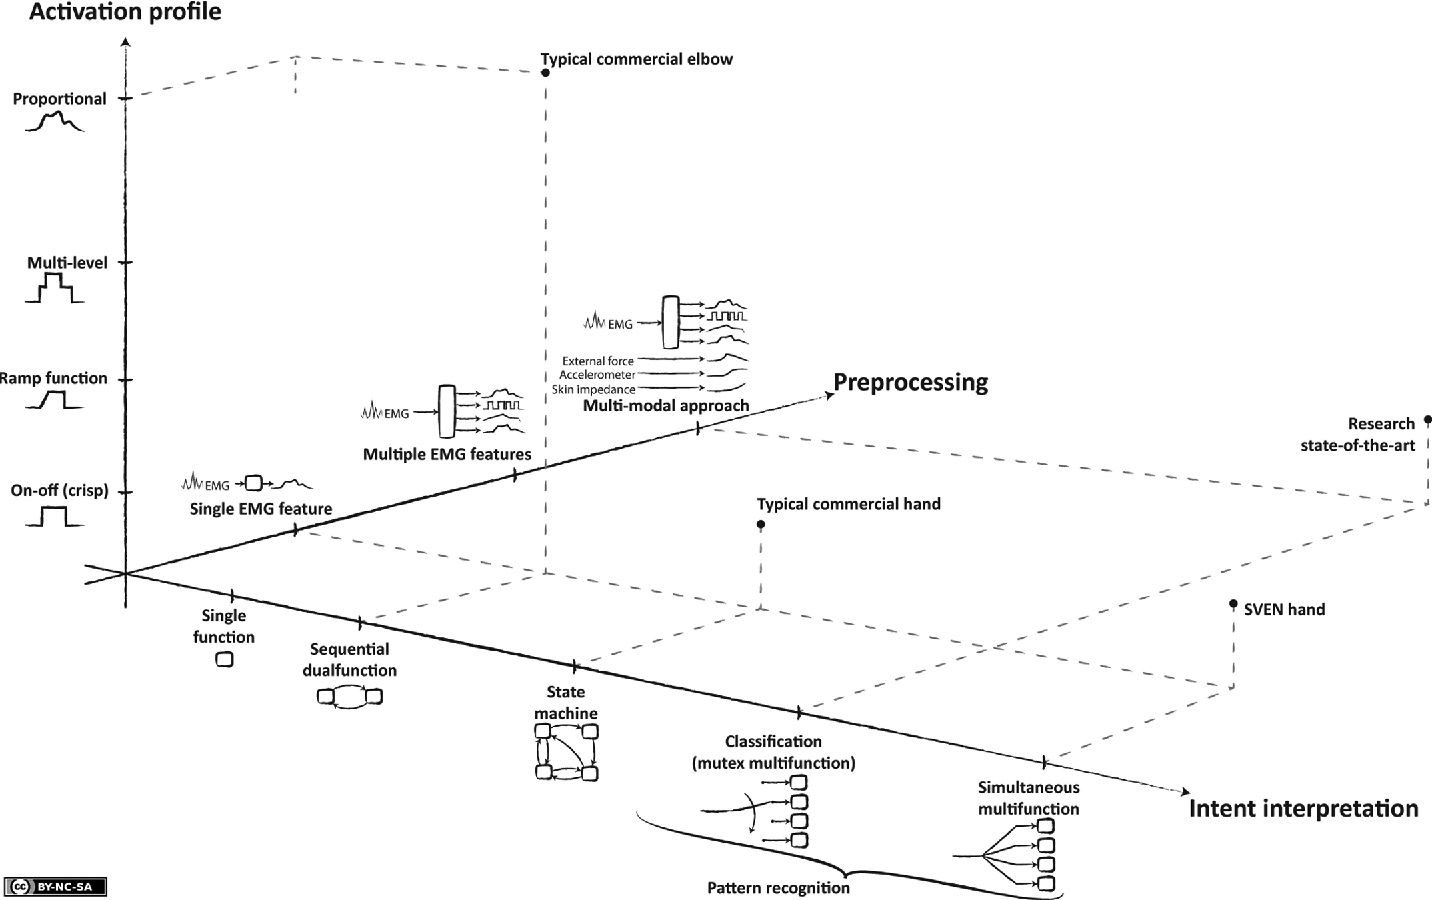
\includegraphics[width=1\textwidth]{Images/myoelectric-control.png}
    \caption{Research state-of-the-art of myoelectric control in the year 2012 [\cite{Fougner2012ControlOU}]}
    \label{fig:myo-control-schema}
\end{figure}
Electromyography (EMG) is an electrodiagnostic technique for evaluating and recording the electrical activity produced by skeletal muscles [\cite{0736093400}]. EMG is performed using an electromyograph which detects the electric potential generated by muscle cells when they are electrically or neurologically activated.
This electric potential can be approximatively considered proportional to the force of the muscle activation.
Due to the preference for noninvasive prostheses, surface EMG (sEMG) signals have been used for the control of upper limb prostheses prosthetic devices since 1948, as testified in \cite{Zecca2002}.
The signal produced by the sEMG sensors are fed to machine learning methods in order to control the prostheses: different machine learning models are used in union to different numbers of sEMG sigmals in order to achieve different level of control on the prostheses. A graphical representation of the different control methods and level, considering also non-machine learning methods, can be found in figure \ref{fig:myo-control-schema}.
In this thesis we work on a myoelectric control system characterized by a \textit{proportional} activation profile, a \textit{simultaneous multifunction} intent interpretation and we consider as input \textit{multiple EMG features}.
\section{Formal Methods}\label{sec:decproc}
Formal methods are a kind of system design techniques which use meticulous mathematical models for the specification, development and verification of software and hardware systems. The application of these kind of methods to the design of both software and hardware systems is supported by the increased reliability and robustness of the resulting systems. In this thesis we are more interested in the use of formal methods as verification techniques: we will consider a finished system and we will try to use the verification techniques in order to enhance its reliability.
In particular the system we will consider is a machine learned controller, therefore in this section we present two of the most popular formal verification techniques used in the verification of machine learning systems: Satisfiability (SAT) and Satisfiability Modulo Theories (SMT).
\subsection{Satisfiability (SAT)}
\begin{figure}[ht]
    \centering
    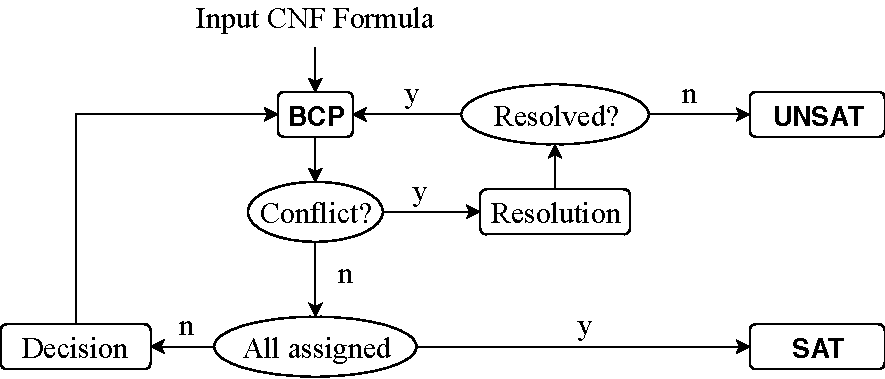
\includegraphics{Images/SAT.pdf}
    \caption{The CDCL framework.}
    \label{fig:cdcl-frame}
\end{figure}
SAT solving aims to check the satisfiability of a propositional logic formula $\varphi$ represented as Boolean combinations of atomic (Boolean) propositions. We introduce CDCL-style SAT solving algorithm, being the most commonly implemented in state-of-the-art SAT solvers.
The CDCL algorithm starts from a CNF formula and then explores the search space by iteratively assigning truth values to some propositions which are chosen according to some heuristic. After each of these assignment the algorithm applies Boolean Constraint Propagation (BPC) to determine the variable assignments implied by the last decision. If the application of BPC leads to a conflict, which is, if the value of a variable is implied to be both true and false at the same time, then \textit{conflict-driven clause-learning} and \textit{non-chronological backtracking} are employed: the algorithm follows back the chain of implication and applies resolution to infer a reason for the conflict in the form of a conflict clause, which then is added to the clause set of the solver. Backtracking removes previous decisions and their implications until the conflict clause can be satisfied. If the starting CNF formula has clauses consisting of a single literal, the algorithm assign them directly. As consequence the algorithm starts with BCP in order to detect implication. If the application of BCP brings to a conflict, the algorithm tries to resolve such conflict. If the conflict is unsolvable then the CNF formula is unsatisfiable, otherwise the algorithm backtracks and continues with BCP. If BCP is completed without conflicts and there are still unassigned propositions, the algorithm makes a new decision. Otherwise the CNF formula is satisfiable and a solution is found.
%
\subsection{Satisfiability Modulo Theories (SMT)}
\begin{figure}[ht]
    \centering
    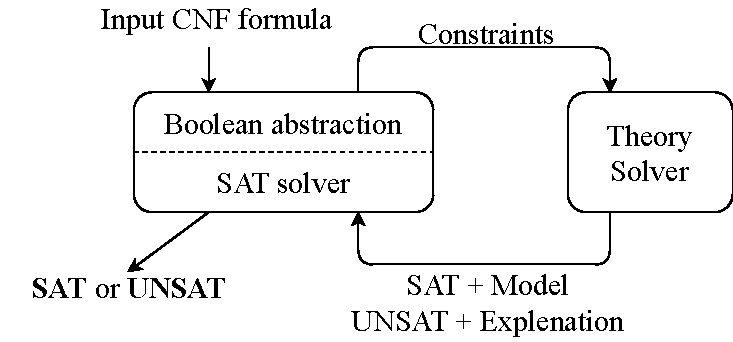
\includegraphics{Images/SMT.pdf}
    \caption{The SMT solving framework.}
    \label{fig:smt-frame}
\end{figure}
Satisfiability Modulo Theories is the problem of deciding the satisfiability of a first-order formula with respect to some decidable theory $\mathcal{T}$. In particular, SMT generalizes the boolean satisfiability problem (SAT) by adding background theories such as the theory of real numbers, the theory of integers, and the theories of data structures (\textit{e.g.}, lists, arrays and bit vectors). To decide the satisfiability of a CNF formulas $\varphi$, SMT solvers usually build a boolean abstraction $\textit{abs}(\varphi)$ by replacing each constraint by a new boolean proposition.
\begin{eqnarray*}
\arraycolsep=2pt
\begin{array}{ccccccccccc}
\varphi &: &\underbrace{x \geq y} &\wedge &(&\underbrace{x > 2}& \vee &\underbrace{y >0}&)& \wedge &\underbrace{y \leq 0} \\
\textit{abs}(\varphi)&:&A& \wedge& (&B& \vee &C&)& \wedge  &\neg C
\end{array}
\label{eq:abs}
\end{eqnarray*}
In the example above $x$ and $y$ are real-valued variable whereas $A$, $B$ and $C$ are boolean proposition.
Once the boolean abstraction is built a SAT solver search for a satisfying assignment $\mu$ for $\textit{abs}(\varphi)$ (e.g. $\mu(A) = \bot$, $\mu(B) = \top$, $\mu(C) = \bot$), if there is no satisfying assignment the CNF formula is unsatisfiable. Otherwise the SMT solver needs to check if the assignment is consistent also in the underlying theory using a \textit{theory solver}. If the theory solver comfirm the consistency of the assignment then a satisfying solution (\textit{model}) is found for $\varphi$. Otherwise the theory solver provides a set of falsified clauses $\phi_T$ which gives an explenation for the conflict, such set is then used to refine the boolean abstraction $\textit{abs}(\varphi)$ to $\textit{abs}(\varphi)\wedge \textit{abs}(\phi_T)$. These steps are iteratively executed until either a theory-consistent Boolean assignment is found, or no more Boolean satisfying assignments exist.
\section{Machine Learning}\label{sec:ML}
The machine learning methods we will consider in this thesis is Ridge Regression with Random Fourier Features (RR-RFF), in the following we will briefly explain the above-mentioned model.
The simplest form of regression is the least square regression:
\begin{equation}
    f(\mathbf{x}) = \mathbf{w}^T\mathbf{x}
    \label{eq:lsr}
\end{equation}
where $\mathbf{w}$ is a weight vector and $\mathbf{x}$ is the input feature vector.
The optimal values for the elements of the vector $\mathbf{w}$ can be found through the minimization of the sum of the squared error between the prediction $f(\mathbf{x})$ and the correct target label $y$. The resulting optimization problem is:
\begin{equation}
    \underset{\mathbf{w}}{arg\,min} \sum_{i=1}^{n} (y_i - f(\mathbf{x}_i))
    \label{eq:lsrmin}
\end{equation}
where $n$ is the number of training samples and $y_i$ is the target label corresponding to the sample $\mathbf{x}_i$. The closed form solution of this optimization problem can easily be found by differentiating equation \ref{eq:lsrmin} with respect to $\mathbf{w}$, setting the result equal to zero and solving the resulting equation for $\mathbf{w}$. The resulting closed form solution is:
\begin{equation}
    \hat{\mathbf{w}} = (\mathbf{X}^T \mathbf{X})^{-1} \mathbf{X}^T \mathbf{y}
    \label{eq:closedlsr}
\end{equation}
where $\mathbf{X} \in \mathbb{R}^{n \times d}$, $n$ is the number of training samples and $d$ is the number of input features. In order to limit the overfitting of the model and, as consequence, achieve a more stable model, a regularisation term can be used. This term leads to a penalization on the values of the weights and therefore to a smoother model. This particular kind of regression is known as Ridge Regression (RR) [\cite{hoerl1970ridge}], the minimization problem becomes:
\begin{equation}
    \underset{\mathbf{w}}{arg\,min} \,\, \frac{1}{2} \sum_{i=1}^{n} (y_i - f(\mathbf{x}_i)) + \frac{\lambda}{2} ||\mathbf{w}||^2
    \label{eq:lsrminreg}
\end{equation}
where $\lambda$ is a strictly positive hyperparameter which scales the contribution of the regularization parameter in the equation. The closed form solution for Ridge Regression can be easily found following the same step used for the standard least square regression.
\begin{equation}
    \hat{\mathbf{w}} = (\mathbf{X}^T \mathbf{X} + \lambda \mathbf{I})^{-1} \mathbf{X}^T \mathbf{y}
    \label{eq:closedrr}
\end{equation}
where $\mathbf{I} \in \mathbb{R}^{d \times d}$ is the identity matrix.
Ridge Regression is a linear model: to extend its application to nonlinear dataset, we can map the input space to a higher dimensional space using a nonlinear basis function $\mathbf{\phi}$:
\begin{equation}
    f(\mathbf{x}) = \mathbf{w}^T\mathbf{\phi}(\mathbf{x})
    \label{eq:fmrr}
\end{equation}
\begin{equation}
    \hat{\mathbf{w}} = (\mathbf{\Phi}^T \mathbf{\Phi} + \lambda \mathbf{I})^{-1} \mathbf{\Phi}^T \mathbf{y}
    \label{eq:closedfmrr}
\end{equation}
where $\mathbf{\Phi} := \mathbf{\Phi}(\mathbf{X}) \in \mathbb{R}^{n \times D}$ and $\mathbf{I} \in \mathbb{R}^{D \times D}$, the number of basis function $D$ is a new hyperparameter of the model.\\
In this thesis we have followed in the step of the work done in \cite{Strazzulla2017} and therefore we have chosen Random Fourier Features (RFF) as basis function:
\begin{equation}
    \phi_{RFF}(\mathbf{x}) = \sqrt{2} \cdot cos(\sigma \cdot \mathbf{\Omega} \cdot \mathbf{x} + \beta)
    \label{eq:rff}
\end{equation}
\begin{equation}
    \mathbf{\Phi} = \mathbf{\Phi}_{RFF}(\textbf{X}) = \sqrt{2} \cdot cos(\mathbf{X} \cdot (\sigma \cdot \mathbf{\Omega})^T + \beta)
    \label{eq:matrff}
\end{equation}
where $\mathbf{\Omega} \in \mathbb{R}^{D \times d}$, $\beta \in \mathbb{R}^D$, $\mathbf{\Omega} \sim \mathcal{N}(0,\,1)$ and $\beta \sim \mathcal{U}(0, 2\pi)$ and $\sigma$ is an hyperparameter which scales the frequency of the distribution.
\chapter{Preliminaries}\label{ch:preliminaries}
In the following we present the control system currently used at DLR, the hardware used with it and the software out-of-the-shelf we have used in the development of our algorithm. We also present the reliability problem we have tried to solve with the above-mentioned algorithm. 
\section{Interactive Myocontrol}\label{sec:interactivemyocontrol}
It is the control system currently used at DLR, it provides a graphical interface for the training and management of the different machine learned controller for different kind of prosthetic hands. For our work we have used the machine learned controller based on the method Ridge Regression with Random Fourier Features (RR-RFF), which we have presented in section \ref{sec:ML}. Given the scope of our work we have decided to use, instead a real prosthetic hand, a virtual model of a prosthetic hand which, when connected with Interactive Myocontrol, reproduce accurately the movement signaled by the controller.
\begin{figure}[ht]
    \centering
    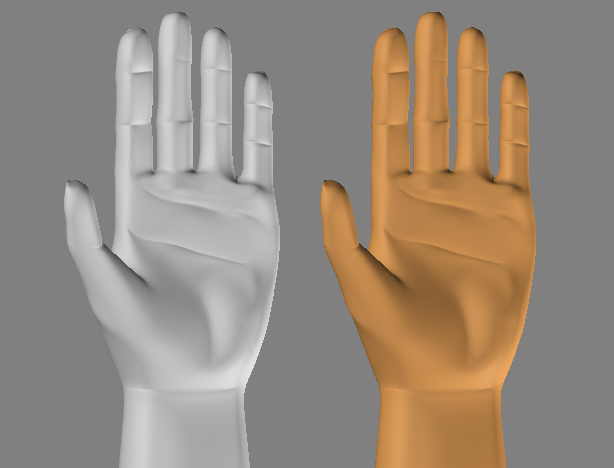
\includegraphics[width=0.5\textwidth]{Images/Blender.PNG}
    \caption{Virtual model of a prosthetic hand used with Interactive Myocontrol. The gray hand is used to reproduce the reference signals, whereas the orange hand is used to reproduce the predictions.}
    \label{fig:hand-blender}
\end{figure}
The hardware used to generate the sEMG signals from the muscular activation of human participants is the Myo Armband manufactured by Thalmic Labs (\href{https://www.thalmic.com}{https://www.thalmic.com}), is provided with eight sEMG sensors uniformly distributed along the bracelet.
\begin{figure}[ht]
    \centering
    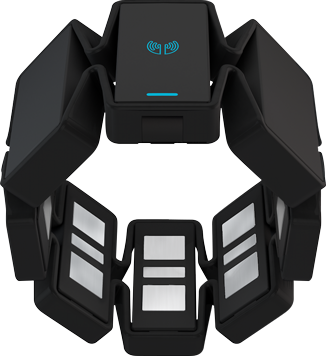
\includegraphics[width=0.5\textwidth]{Images/myo_armband.png}
    \caption{Myo Armband manufactured by \href{https://www.myo.com/techspecs}{Thalmic Labs}}
    \label{fig:myo_armband}
\end{figure}
The sEMG signals produced by the bracelet are the only input signal used by our machine learned controller, before being passed as input to the controller the signals are rectified and mildly low-pass filtered with a 2nd order Butterworth filter (cutoff 1Hz).
The outputs of the machine learned controller are nine different value which corresponds to the activation level of the nine different degrees of freedom (DOFs) of the prosthetic hand. In a real prosthetic hand these nine values are used to directly control the actuators which permits the movement of the hand, whereas in our case these values are used to control the position of the virtual model of the hand. Interactive Myocontrol use the different values of the nine DOFs to define 17 different action that are used as references in the training of the controller. In this work we are only interested in four of these actions, which are: rest, power grasp, wrist flexion and wrist extension; for convenience's sake we will consider as outputs the activation level of the above mentioned actions.
Interactive Myocontrol let the user decide which subset of the 17 actions desires to use in the training of the machine learned controller.
Therefore each sample of the training set $S$ is composed of an input sample $\mathbf{x}_i \in \mathbb{R}^8$ and a corresponding target value $\mathbf{y}_i \in \mathbb{R}^9$. In particular, given the physical limits of the sEMG sensors, each features of the input samples is limited between 0 and 5, therefore we can further limit the input space to $[0, 5]^8$.
As is customary in the current state of the art (see, eg., \cite{hahne2015concurrent}, \cite{sierra2013realistic}) in practice $S$ is built by gathering for each action of interest a certain number of observations while the participant is doing that particular action; each observation is then coupled with the target value associated to the action.
For example, the participant is asked to power grasp ("make a fist"); once the experimenter verifies that the signals have reached a stable pattern, well distinct from the baseline, a suitable number of observations is recorded and associated to (synthetic) target values denoting maximal activation of all fingers. This methodology is called on-off goal-directed training.
Interactive Myocontrol permits an incremental training of the machine learned controller: it is possible for the user to add new training samples after the initial training session and retrain the learning machine using also the new data; in \cite{Strazzulla2017} such machine learned controller is called \textit{Incremental-Learning Myoelectric Controller}
\section{dReal}\label{sec:dReal}
In this work we needed an SMT solver which could manage trascendent functions, due to the utilization of the Random Fourier Features as feature map in the machine learned controller. We chose dReal \cite{gao2013dreal} because it satisfied our requirements and was provided with an API python which could be easily used in our code. It was out of the scope of this thesis to compare the performance of different SMT solver, therefore we didn't consider others than dReal.
In order to handle a wide range of nonlinear real functions dReal implements the framework of $\delta$-complete decision procedures. We say a decision procedures is $\delta$-complete for a set of formulas $S$ if for any $\phi \in S$ the procedure returns \textit{unsat} if $\phi$ is unsatisfiable or \textit{$\delta$-sat} if $\phi^\delta$ is satisfiable.
$\delta$ is an arbitrary positive rational number and $\phi^\delta$ is a syntactic variant of $\phi$ that encodes a notion of numerical perturbation on logic formulas. Essentialy we relax the constrains on the procedure in order to permit answers with an one sided $\delta$-bounded error, therefore $\delta$-complete decision procedures can exploit the power of numerical approximations without losing formal correctness guarantees.
\chapter{Conclusion and Future Work}\label{c:conclusion}
HERE CONCLUSION

\bibliographystyle{abbrv}
\bibliography{mybib.bib}
\end{document}
